\section{From matching factors to low-degree squares}
\label{sec:matching}

We now combine the three ingredients: the local restrictions of
Lemma~\ref{lem:local-averaging}, the product averaging result in
Theorem~\ref{thm:fourier-smoothing}, and the separating functional from
Proposition~\ref{prop:parity-functional}.  The vertices of the parity
graph will become cells of matching vertices.  Averaging the row factor
within each cell realizes the parity disagreement function exactly.
The Fourier estimate will then approximate that function by squares
on which the separating functional is nonnegative.

\begin{lemma}[Normalization of PSD factors]
\label{lem:normalization}
Let $S$ be a finite nonzero nonnegative matrix with entries at most $B$.
If $S$ admits a real PSD factorization of size $r_0$, it admits one
of size $r\le r_0$ whose row factors $F_a$ and column factors $G_m$
satisfy
\[
 \tr F_a\le B,\qquad \tr G_m\le r.
\]
\end{lemma}
\begin{proof}
Compress to the span of the images of all column factors.  This
preserves their pairings with the row factors and reduces the size
to some $r\ge1$.  The average column factor is positive definite on
this span.  Hence the compact convex hull of the column factors
contains a positive definite matrix $J$ maximizing the determinant.
The one-sided derivative of $\log\det$ in the direction $G_m-J$
is nonpositive, giving
\[
 \tr(J^{-1}G_m)\le r.
\]
Replace the column factors by $J^{-1/2}G_mJ^{-1/2}$ and the row
factors by $J^{1/2}F_aJ^{1/2}$.  These congruences preserve PSD and
trace pairings.  The new column traces have the required bound.
The new row trace is $\tr(F_aJ)$, a convex combination of entries
of the original row, and is at most $B$.
\end{proof}

\begin{proof}[Proof of Theorem~\ref{thm:main}]
Use the constants $d=100$, $\beta=1/100$, and $\tau=1/1000$ of
Section~\ref{sec:parity}, and put $L=2^{d-1}$.  Let $C_L$ be the
constant in Lemma~\ref{lem:splitting}.  First choose $\lambda>1$
so that
\begin{equation}\label{eq:matching-lambda}
 \lambda^\tau\ge64L^4.
\end{equation}
Next fix an even integer $k$ large enough for the local construction
and for
\begin{equation}\label{eq:matching-local-smallness}
 L\lambda^2C_L\theta_d(k)\le1.
\end{equation}
Lemma~\ref{lem:local-averaging} permits this choice.  These constants
are fixed independently of $n$ and $\rho$.

Fix $0<\rho<1$ and set $\epsilon=1-\rho$.  For a large even $n$,
let $t$ be the largest even integer satisfying $kt\le n$.  Then
\begin{equation}\label{eq:matching-size}
 kt\le n<k(t+2).
\end{equation}
Take a $d$-regular bipartite multigraph $H$ on $t$ vertices as in
Lemma~\ref{lem:expander}, and give its vertices charges $b_i\in\{0,1\}$,
with exactly one charge equal to one.  Order the $d$ incidences at
each vertex.  Write $Y_i$ for the parity-$b_i$ incidence assignments,
identified with the Boolean group on their first $d-1$ bits.

\paragraph{Realizing the restrictions by matchings.}
Partition $kt$ vertices of $K_n$ into cells $C_1,\ldots,C_t$ of
size $k$.  The remaining vertices have even cardinality and will
be paired in a fixed way.  In cell $i$, choose the unique weight
$w_i\in\{k/2,k/2+1\}$ of parity $b_i$, and let $X_i$ be the
$w_i$-subsets of $C_i$.  For $a=(a_1,\ldots,a_t)\in\prod_iX_i$,
use the odd-cut row
\[
 U(a)=\bigcup_i a_i.
\]
It is odd because $|U(a)|\equiv\sum_i b_i\equiv1\pmod2$.

In each cell independently, sample the local column data $m_i$
of Section~\ref{sec:local}: $d$ ordered distinct terminals and a
pairing of the other vertices.  For every auxiliary edge $e=uv$,
match the terminal at its incidence in $C_u$ to the terminal at
its incidence in $C_v$.  Together with the internal pairings and
the fixed remainder pairing, this gives a perfect matching $M(m)$.
Parallel edges in $H$ use distinct terminals, so they cause no
conflict.  Distinct local data need not give distinct matchings;
we simply use the factor of the matching they specify.

For $y=(y_1,\ldots,y_t)\in\prod_iY_i$, apply the local laws
$\pi_{y_i}^{m_i}$ independently.  An internal pair has equal cut
bits and contributes no crossing.  The matched remainder is
outside $U(a)$.  An intercell edge crosses exactly when its two
terminal bits disagree, as illustrated in
Figure~\ref{fig:matching-cells}.  Thus every cut in the support
of the product restriction satisfies
\begin{equation}\label{eq:matching-realization}
 |M(m)\cap\delta(U(a))|-1+\rho
 =\sum_{e=uv\in E(H)}\mathbf1_{\{y_{u,e}\ne y_{v,e}\}}-\epsilon
 =f(y).
\end{equation}

\begin{figure}[tbp]
\centering
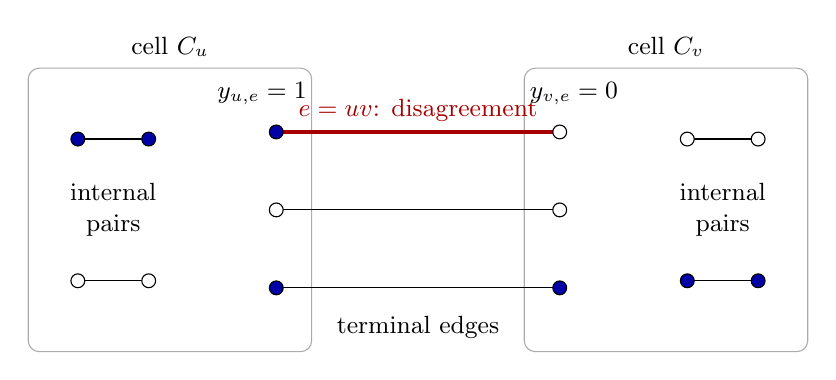
\begin{tikzpicture}[x=.9cm,y=.9cm,font=\small]
 \tikzset{bit/.style={circle,draw,minimum size=5pt,inner sep=0pt},
  one/.style={bit,fill=blue!65!black},zero/.style={bit,fill=white}}
 \draw[rounded corners,gray!65] (0,0) rectangle (4,4);
 \draw[rounded corners,gray!65] (7,0) rectangle (11,4);
 \node at (2,4.3) {cell $C_u$};
 \node at (9,4.3) {cell $C_v$};
 \draw (.7,3)--(1.7,3) (.7,1)--(1.7,1);
 \draw (9.3,3)--(10.3,3) (9.3,1)--(10.3,1);
 \node[one] at (.7,3) {}; \node[one] at (1.7,3) {};
 \node[zero] at (.7,1) {}; \node[zero] at (1.7,1) {};
 \node[zero] at (9.3,3) {}; \node[zero] at (10.3,3) {};
 \node[one] at (9.3,1) {}; \node[one] at (10.3,1) {};
 \node[align=center] at (1.2,2) {internal\\pairs};
 \node[align=center] at (9.8,2) {internal\\pairs};
 \draw[very thick,red!65!black] (3.5,3.1)--(7.5,3.1)
  node[midway,above] {$e=uv$: disagreement};
 \draw (3.5,2)--(7.5,2) (3.5,.9)--(7.5,.9);
 \node[one] at (3.5,3.1) {}; \node[zero] at (7.5,3.1) {};
 \node[zero] at (3.5,2) {}; \node[zero] at (7.5,2) {};
 \node[one] at (3.5,.9) {}; \node[one] at (7.5,.9) {};
 \node[above] at (3.3,3.35) {$y_{u,e}=1$};
 \node[above] at (7.7,3.35) {$y_{v,e}=0$};
 \node at (5.5,.35) {terminal edges};
\end{tikzpicture}

\caption{Part of the matching associated with two cells.  Filled vertices
belong to the cut and open vertices do not.  The restriction gives equal
bits to each internal pair, so only terminal edges can cross.  The
highlighted edge corresponds to a disagreement at an auxiliary edge
$e=uv$.  Only a few of the $d$ terminals and internal pairs are shown.}
\label{fig:matching-cells}
\end{figure}

\paragraph{A factorization and its Fourier approximation.}
Suppose that $A_n(\rho)$ has a PSD factorization of size at most
$2^t$.  Its entries are positive and at most $n$.
Lemma~\ref{lem:normalization} gives factors of size $r\le2^t$ with
\[
 \tr F_U\le n,\qquad \tr G_M\le r.
\]
Put $F(a)=F_{U(a)}$.  For any fixed local column data $m$, let
$\overline F_m(y)$ be the product-restricted average of $F$.
Equation~\eqref{eq:matching-realization} gives the exact identity
\begin{equation}\label{eq:matching-pairing}
 \tr\bigl(\overline F_m(y)G_{M(m)}\bigr)=f(y).
\end{equation}

Apply Theorem~\ref{thm:fourier-smoothing} with the local channels
above, the trace bound $B=n$, and
Equation~\eqref{eq:matching-local-smallness}.  It gives a choice of
$m$ and rectangular matrix functions $H_q$, indexed by
$q\in\Lambda^t$, such that
\begin{align}
 \overline F_m(y)&=\sum_q H_q(y)^{\mathsf T}H_q(y),
 \label{eq:matching-squares}\\
 \sum_{q,p}\lambda^{\dist(q,p)}\normF{\widehat H_{q,p}}^2
 &\le L^t\sqrt r\,n2^{t/2}.
 \label{eq:matching-fourier-bound}
\end{align}
Here $\Lambda$ is the character group on $d-1$ free bits, and
$\dist$ counts differing blocks.  Fix these data and set
$G=G_{M(m)}$.  By Equations~\eqref{eq:matching-pairing} and
\eqref{eq:matching-squares},
\begin{equation}\label{eq:matching-full-squares}
 f(y)=\sum_q\normF{H_q(y)G^{1/2}}^2.
\end{equation}

Let $D=\lfloor\tau t\rfloor$.  In branch $q$, retain only the
Fourier coefficients at distance at most $D$ from $q$, writing
\[
 K_q(y)=\sum_{p:\,\dist(q,p)\le D}\widehat H_{q,p}\chi_p(y),
 \qquad
 f_*(y)=\sum_q\normF{K_q(y)G^{1/2}}^2.
\]
The sum of squared norms of the discarded matrices at any $y$ is
at most
\begin{align}
 E_t(y)^2
 &:=\sum_q\normF{(H_q(y)-K_q(y))G^{1/2}}^2\notag\\
 &\le L^t\sum_{q,p:\,\dist(q,p)>D}
                    \normF{\widehat H_{q,p}G^{1/2}}^2\notag\\
 &\le L^t r\lambda^{-\tau t}
              \bigl(L^t\sqrt r\,n2^{t/2}\bigr)\notag\\
 &\le n\left(\frac{4L^2}{\lambda^\tau}\right)^t
 \le n(4L)^{-2t}.
 \label{eq:matching-tail}
\end{align}
The first inequality is Cauchy--Schwarz over at most $L^t$
characters in each branch.  The second uses
$\normop G\le\tr G\le r$, Equation~\eqref{eq:matching-fourier-bound},
and the fact that an integer distance greater than $D$ is greater
than $\tau t$.  The last line uses $r\le2^t$ and
Equation~\eqref{eq:matching-lambda}.

The full stack in Equation~\eqref{eq:matching-full-squares} has norm
at most $\sqrt n$.  Expanding the difference of the squared norms
of that stack and its truncation, and then using
Equation~\eqref{eq:matching-tail}, gives
\begin{equation}\label{eq:matching-uniform-error}
 \norm{f-f_*}_\infty
 \le 2n(4L)^{-t}+n(4L)^{-2t}.
\end{equation}

\paragraph{The separating functional.}
In branch $q$, multiplication by the real character $\chi_q$
does not change any square.  It translates a retained frequency
$p$ to $p+q$, whose block degree is $\dist(p,q)\le D$.
This character translation is the elementary support-shifting
principle used in Fourier sums of squares
\cite{fsp-sparse}.
Consequently $f_*$ is a sum of squares of real functions of block
degree at most $D$, including after multiplication by the constant
matrix $G^{1/2}$.

Proposition~\ref{prop:parity-functional} therefore supplies a
functional $\mathcal D$ with
\[
 \mathcal D(f_*)\ge0,\qquad \mathcal D(f)=-\epsilon.
\]
On the other hand, its norm bound and
Equation~\eqref{eq:matching-uniform-error} give
\[
 |\mathcal D(f-f_*)|
 \le 2n4^{-t}+n(16L)^{-t}\longrightarrow0
\]
by Equation~\eqref{eq:matching-size}, since $k$ is fixed.
For sufficiently large $n$, this is smaller than $\epsilon$,
a contradiction.

We have excluded every factorization of size at most $2^t$.
For all sufficiently large $n$, Equation~\eqref{eq:matching-size}
also gives $t\ge n/(2k)$.  Thus
\[
 \rankpsd A_n(\rho)>2^t\ge2^{n/(2k)}.
\]
Taking $c=1/(2k)$ proves the theorem.  Only the final comparison
with $\epsilon=1-\rho$ makes the threshold depend on $\rho$.
\end{proof}
